
\chapter{Introduction to Numerical Methods relevant to Thermodynamics}\label{Appendix_NumMethods}

{\it This is not examinable} -- it is here so that you can see where some of the notations, operations and results of earlier sections came from. Details of the contents of this Appendix can be found in \cite{Atkinson_Book_Newton,Atkinson_Book_Interpolation,NumericalRecipes_Interpolation,NumericalRecipes_Newton} or in any text-book of {\it Mathematical or Numerical Methods} for engineering.

%%%
%%% SECTION
%%%
\section{Linear Interpolation}\label{LinearInterpolation}\index{Linear interpolation}

Given a continuous and unknown function $f(x)$, defined at a set of points  $x_{1} < \cdots < x_{i} < \cdots < x_{N}$. Interpolation is the process of determining a polynomial expression to calculate the pair $\left[x_{k}, f\left(x_{k}\right)\right]$ based on neighbours discrete coordinates $\left\{\left[x_{1},f\left(x_{1}\right)\right], \cdots, \left[x_{N},f\left(x_{N}\right)\right]\right\}$. 

Consider a set of discrete data points,
  \begin{center}
    \begin{tabular}{c | c }
        $\mathbf{x}$   & $\mathbf{f\left(x_{i}\right)}$ \\
        \hline
           $x_{1}$ &  $f\left(x_{1}\right)$ \\
           $x_{2}$ &  $f\left(x_{2}\right)$ \\
           $x_{3}$ &  $f\left(x_{3}\right)$ \\
           $x_{4}$ &  $f\left(x_{4}\right)$ \\
    \end{tabular}
  \end{center}
that are a subset of a continuous and smooth function $y=f(x)$ (Fig.~\ref{Appendix:Fig:Interpolation}). Polynomials of order $n\ge 1$ can be generated to represent this function. High-order polynomials can more accurately fit the discrete coordinatess than low-order polynomials. In Fig.~\ref{Appendix:Fig:Interpolation}, let's assume the discrete pairs 
  \begin{displaymath}
     \left\{\left[x_{1},f\left(x_{1}\right)\right], \left[x_{2},f\left(x_{2}\right)\right],\left[x_{3},f\left(x_{3}\right)\right], \left[x_{4},f\left(x_{4}\right)\right]\right\}
  \end{displaymath}
are known, and one wants to determine the value of the function $f$ at $x_{2} < x_{k} < x_{3}$. If the interval $\Delta x= x_{3}-x_{2}$ is sufficiently small, a linear function can be used to fit these coordinates,
   \begin{equation}
       f\left(x_{k}\right) = f\left(x_{2}\right) + m\left(x_{k}-x_{2}\right),\label{LinearInterpolation:Eqn1}
   \end{equation}
where 
   \begin{displaymath}
      m = \frc{f\left(x_{3}\right)-f\left(x_{2}\right)}{x_{3}-x_{2}}.
   \end{displaymath}
If $m$ is replaced in Eqn.~\ref{LinearInterpolation:Eqn1},
   \begin{displaymath}
       f\left(x_{k}\right) = \frc{f\left(x_{2}\right)\left(x_{3}-x_{k}\right) + f\left(x_{3}\right)\left(x_{k}-x_{2}\right)}{x_{3}-x_{2}}.
   \end{displaymath}
   
   \begin{shaded}
      Or for a general case with $x_{a} < x_{k} < x_{b}$,
        \begin{equation}\label{LinearInterpolation:Eqn1}
            f\left(x_{k}\right) = \frc{f\left(x_{a}\right)\left(x_{b}-x_{k}\right) + f\left(x_{b}\right)\left(x_{k}-x_{a}\right)}{x_{b}-x_{a}}.
        \end{equation}
   \end{shaded}

%%% Figure
     \begin{figure}[h]\label{Appendix:Fig:Interpolation}%
        \begin{center}
          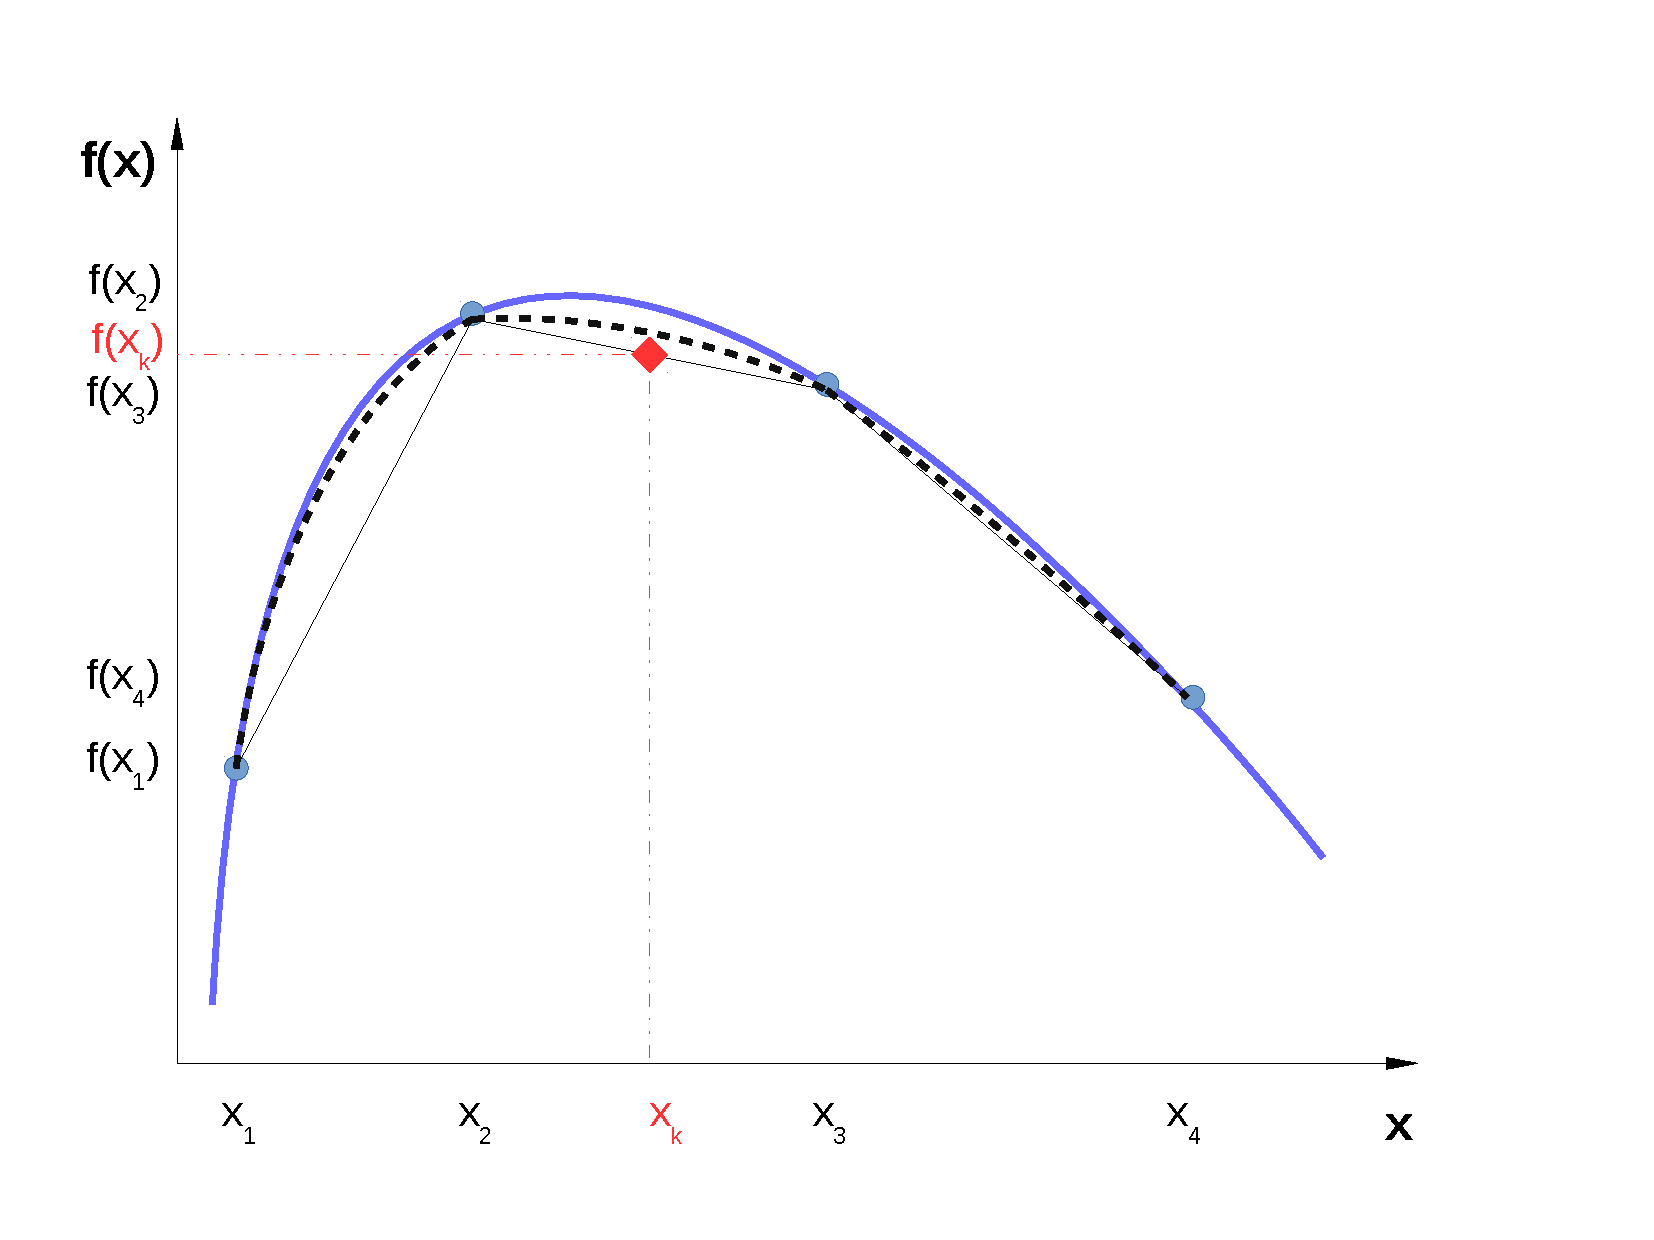
\includegraphics[width=\columnwidth,clip]{./Pics/Interpolation}
           \caption{Smooth function $f(x)$ (solid blue line) may be more accurately interpolated by a high-order polynomial (black dotted line) than by a low-order polynomial (solid black line).} 
        \end{center}
      \end{figure}

    \begin{list}{\bf Example \arabic{qcounter}:~}{\usecounter{qcounter}}
%       
         \item Given a table of values for $f(x)=\tan{x}$ for a few values of $x$,
            \begin{center}
               \begin{tabular}{c | c c c c}
                   $x$        & 1.00   & 1.10   & 1.20   & 1.30   \\
                   \hline
                   $\tan{x}$  & 1.5574 & 1.9648 & 2.5722 & 3.6021 \\
               \end{tabular}
            \end{center}
            Estimate $\tan{1.15}$ and $\tan{1.23}$.

            {\bf Solution:} For $\left(x_{a}=1.10\right) < \left(x_{k}=1.15\right) < \left(x_{b}=1.20\right)$,
               \begin{eqnarray}
                  f\left(x_{k}\right) &=& \frc{f\left(x_{a}\right)\left(x_{b}-x_{k}\right) + f\left(x_{b}\right)\left(x_{k}-x_{a}\right)}{x_{b}-x_{a}} \nonumber \\
                                     &=& \frc{1.9648\times(1.20-1.15) + 2.5722\times(1.15-1.10)}{1.20-1.10} = 2.2685 \nonumber
               \end{eqnarray}

For  $\left(x_{a}=1.20\right) < \left(x_{k}=1.23\right) < \left(x_{b}=1.30\right)$,
               \begin{eqnarray}
                  f\left(x_{k}\right) &=& \frc{f\left(x_{a}\right)\left(x_{b}-x_{k}\right) + f\left(x_{b}\right)\left(x_{k}-x_{a}\right)}{x_{b}-x_{a}} \nonumber \\
                                     &=& \frc{2.5722\times(1.30-1.23) + 3.6021\times(1.23-1.20)}{1.30-1.20} = 2.8812 \nonumber
               \end{eqnarray}
%
         \item Calculate specific volume $\left(v, \text{in m}^{3}\text{.kg}^{-1}\right)$ internal energy $\left(u, \text{in kJ.kg}^{-1}\right)$ and entropy $\left(s, \text{in kJ.(kg.K)}^{-1}\right)$ of saturated water vapour at 133.45$^{\circ}$C.

           {\bf Solution:} From Appendix~\ref{Appendix:Saturated_SH_Tables} (Table A-2), for $T_{a}(=130.0) < T_{k} (= 133.45) < T_{b} (=140.0)^{\circ}C$, thus:
               \begin{eqnarray}
                  v\left(T_{k}\right) &=& \frc{v\left(T_{a}\right)\left(T_{b}-T_{k}\right) + v\left(T_{b}\right)\left(T_{k}-T_{a}\right)}{T_{b}-T_{a}} \nonumber \\
                                     &=& \frc{0.6685\times(140.0-133.45) + 0.5089\times(133.45-130.0)}{140.0-130.0} = 0.6134 \text{ m}^{3}\text{.kg}^{-1}\nonumber \\
                                     && \nonumber \\
                  u\left(T_{k}\right) &=& \frc{u\left(T_{a}\right)\left(T_{b}-T_{k}\right) + u\left(T_{b}\right)\left(T_{k}-T_{a}\right)}{T_{b}-T_{a}} \nonumber \\
                                     &=& \frc{2539.9\times(140.0-133.45) + 2550.0\times(133.45-130.0)}{140.0-130.0} = 2543.39 \text{ kJ.kg}^{-1}\nonumber \\
                                     && \nonumber \\
                  s\left(T_{k}\right) &=& \frc{s\left(T_{a}\right)\left(T_{b}-T_{k}\right) + s\left(T_{b}\right)\left(T_{k}-T_{a}\right)}{T_{b}-T_{a}} \nonumber \\
                                     &=& \frc{7.0269\times(140.0-133.45) + 6.9299\times(133.45-130.0)}{140.0-130.0} = 6.9934 \text{ kJ.}\left(\text{kg.K}\right)^{-1}\nonumber 
               \end{eqnarray}


    \end{list}

%%%
%%% SECTION
%%%
\section{Root Finder}

%%% SUBSECTION
\subsection{Motivation}
Given a smooth and {\it continuous} function $f(x)$
